%!TEX root = ./main.tex


\section{5G Toolbox}


% Put these frames into your Beamer file.
\begin{frame}
  \centering
  \Huge
  \textbf{MATLAB 5G Toolbox}\\
  \vspace{0.8em}
  \Large
  Do we still need to build 5G from scratch?
\end{frame}

\begin{frame}
  \begin{columns}
    \column{0.48\textwidth}
      \Huge
      Start from a reference.\\
      \vspace{0.6em}
      \Large
      MATLAB already gives you\\
      a solid 5G NR toolbox.
    \column{0.52\textwidth}
      \centering
      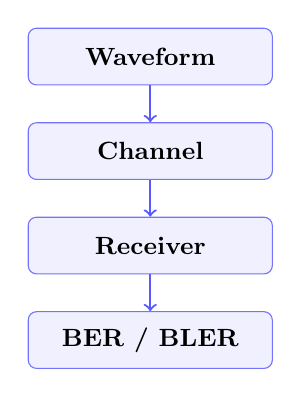
\begin{tikzpicture}[
        box/.style={draw=blue!55, fill=blue!6, rounded corners=3pt, minimum width=3.1cm, minimum height=0.72cm, align=center, font=\small\bfseries},
        arrow/.style={->, thick, blue!65}
      ]
        \node[box] (wave) at (0,1.8) {Waveform};
        \node[box] (chan) at (0,0.6) {Channel};
        \node[box] (recv) at (0,-0.6) {Receiver};
        \node[box] (metric) at (0,-1.8) {BER / BLER};
        \draw[arrow] (wave) -- (chan);
        \draw[arrow] (chan) -- (recv);
        \draw[arrow] (recv) -- (metric);
      \end{tikzpicture}
  \end{columns}
\end{frame}

\begin{frame}{What Is 5G Toolbox?}
% \Large
\begin{itemize}
  \item A MATLAB add-on to \textbf{model, simulate, analyze, and test} 5G communications systems.
  \item Built-in workflows for:
  \begin{itemize}
    \item \textbf{Waveform generation}
    \item \textbf{Link-level simulation}
    \item \textbf{Golden reference design verification}
    \item \textbf{System-level simulation}
  \end{itemize}
  \item \blink{https://www.mathworks.com/products/5g.html}{More details here}
\end{itemize}

\end{frame}

\begin{frame}{Waveforms in Minutes}
% \Large
\begin{itemize}
  \item Generate uplink and downlink waveforms with:
  \begin{itemize}
    \item \textbf{subcarrier spacing}, \textbf{bandwidth parts}, \textbf{frame numerology}
  \end{itemize}
  \item Wireless Waveform Generator app:
  \begin{itemize}
    \item \textbf{NR Test Models (NR-TM)}
    \item \textbf{Downlink Fixed Reference Channels (FRC)}
    \item For \textbf{FR1} and \textbf{FR2}
  \end{itemize}
\end{itemize}
\end{frame}

\begin{frame}{Channels and Signals You Will See in Real 5G}

\begin{itemize}
  \item Physical channels:
  \begin{itemize}
    \item Uplink/downlink shared channels
    \item Control and broadcast channels
  \end{itemize}
  \item Synchronization and reference signals:
  \begin{itemize}
    \item PSS, SSS
    \item DM-RS (demodulation, timing, sync)
    \item Phase tracking, CSI-related reference signals
    \item SRS (sounding reference signal)
    \item PRACH (random access)
  \end{itemize}
\end{itemize}
\end{frame}

\begin{frame}{Link-Level Simulation: The Classic Pipeline}
\begin{itemize}
  \item End-to-end link simulation:
  \begin{itemize}
    \item transmitter $\rightarrow$ channel $\rightarrow$ receiver
  \end{itemize}
  \item Standard channel models:
  \begin{itemize}
    \item \textbf{CDL} and \textbf{TDL} channel models
  \end{itemize}
  \item Metrics you can compute:
  \begin{itemize}
    \item BER, BLER, throughput
  \end{itemize}
  \item Receiver building blocks:
  \begin{itemize}
    \item channel/timing estimation, synchronization, equalization
  \end{itemize}
\end{itemize}
\end{frame}

\begin{frame}{Coding and Procedures Are Included}
\begin{itemize}
  \item Channel coding components:
  \begin{itemize}
    \item \textbf{LDPC} and \textbf{Polar} coding subcomponents
  \end{itemize}
  \item Initial access procedures:
  \begin{itemize}
    \item cell search and selection
    \item decode \textbf{MIB} and \textbf{SIB1}
    \item construct SS bursts and sync using DM-RS
  \end{itemize}
\end{itemize}
\end{frame}

\begin{frame}{System-Level Simulation: Multi-Node, Scheduling}
\begin{itemize}
  \item Multi-node simulations at the system level
  \item Example: \textbf{PUSCH scheduling} under different MAC strategies
  \item Great for understanding:
  \begin{itemize}
    \item RAN behaviors, resource allocation, and performance tradeoffs
  \end{itemize}
\end{itemize}
\end{frame}

\begin{frame}{The Part I Really Want You to Use}
\Large  
\centering
\textbf{It is open MATLAB source code.}\\
\vspace{0.8em}
\Large
Read it like a textbook.
\end{frame}

\begin{frame}{Why This Matters}

\begin{itemize}
  \item You can access features as \textbf{customizable MATLAB source code}.
  \item Treat it as a \textbf{golden reference} for design verification.
  \item If you dissect the implementation step by step (with the help of your GPT teacher),
  \begin{itemize}
    \item you will understand how 5G NR really works.
    \item \textcolor{red}{\textbf{you will become a 5G (6G) engineer faster}}.
  \end{itemize}

\end{itemize}

\end{frame}

